%        File: exam1revAns.tex
%     Created: Wed Feb 06 12:00 PM 2013 P
% Last Change: Wed Feb 06 12:00 PM 2013 P
%
\documentclass[12pt,letterpaper,fleqn]{article}

%       amslatex provides nice math extensions for typesetting mathematics
\usepackage{amsmath}
\usepackage{tmmaths}

%       pstricks provides powerful environments for incorporating postscript into a
%       TeX/LaTeX document. You must have a postscript printer and a package like
%       dvips to convert the DVI file to a PS file.
%\usepackage{pst-all}
%\usepackage{pstricks,pst-plot}
%\usepackage{pst-coil,pst-node}

%   tikz provides high-level language constructs for creating graphics using pgf.
\usepackage{tikz}
%\usetikzlibrary{arrows,snakes,backgrounds}

%  This package provides native tex support for numbered grids. The syntax is:
%  \graphpaper[spc](x_lowleft,y_lowleft)(x_upperright,y_upperright)

%\usepackage{graphpap}
%\usepackage{float}

%  The package below must be initialized with "\initfloatingfigs" immediately after the
%  "\begin{document} command.
%\usepackage{floatfig}

%\usepackage{graphicx}
%\graphicspath{{i:/mytex/graphics}}
%\DeclareGraphicsExtensions{.ps,.eps}

%       tst is a package for the creation of exams, quizzes and tests. the include
%       file mathstuf (see below) provides many abbreviations for these environments.
%\usepackage{tst}

%       epsfig is a package which provides for the inclusion of Encapsulated PostScript
%       files in a document.
%\usepackage{epsfig}
%\usepackage{epic,eepic}
\usepackage[total={7.25in,10in},top=0.25in,left=0.75in,includehead]{geometry}
\usepackage{fancyhdr}
\pagestyle{fancy}
\lhead{Math 253}
%\rhead{\large Name\makebox[2in]{\hrulefill}}
\chead{\LARGE Assignment 1}
%\lfoot{\today}
\cfoot{}
%\rfoot{\thepage}
\renewcommand{\headrulewidth}{0.4pt}
\renewcommand{\footrulewidth}{0.4pt}
\setlength{\parindent}{0pt}
\setlength{\parskip}{2ex}

%\newcounter{tf}[enumi]
%\newenvironment{tf}[0]{\begin{list}%
%{\alph{tf}. \makebox[5em]{True\hfill False}}%
%{\usecounter{tf}\setlength{\labelwidth}{7em}%
%\setlength{\leftmargin}{3.5cm}%
%\setlength{\labelsep}{1cm}}}%
%{\end{list}}

%\usepackage{epic,eepic}
%\newcommand{\numline}{%
%\newcounter{mark}%
%\setcounter{mark}{-1}%
%\setlength{\unitlength}{0.1in}%
%\begin{picture}(0,0)%
%\thicklines%
%\put(0,0){\line(1,0){60}}%
%\multiput(0,0)(10,0){7}{\line(0,-1){1}%
%\makebox(0,-1.5)[t]{\arabic{mark}}\stepcounter{mark}}%
%
%\thinlines%
%\multiput(0,0)(5,0){12}{\line(0,-1){0.5}}%
%\multiput(0,0)(1,0){60}{\line(0,-1){0.3}}%
%\put(-5,265){\makebox(0,0)[l]{{\bf cm}}}%
%\end{picture}}%

\newcommand{\ds}{\displaystyle}
\renewcommand{\deg}{\ensuremath{{}^\circ}}
\let\oldhat\hat
\renewcommand{\hat}[1]{\oldhat{\boldsymbol{\mathbf{#1}}}}
\newcommand{\lv}[1]{\ensuremath{\langle #1 \rangle}}
\newcommand{\ih}{\ensuremath{\hat{\imath}}}
\newcommand{\jh}{\ensuremath{\hat{\jmath}}}
\newcommand{\kh}{\ensuremath{\mathbf{\oldhat{k}}}}
\newcommand{\ora}[1]{\ensuremath{\overrightarrow{#1}}}
\usepackage{tabularx}

\begin{document}
A curve is described by $\vec{r}(t) = \lv{e^t \sin t, e^t \cos t, 0}$. Its graph
over the interval $0 \leq t \leq \frac{3\pi}{2}$ is shown below along with points
spiraling out from $(0,1)$ plotted for $t$ values of $0, \pi/3, 2\pi/3, \pi
 \text{ and } 4\pi/3$.\\
\begin{figure}[!htb]
 \centering
 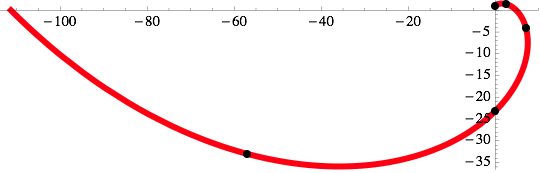
\includegraphics[width=0.5\textwidth]{img/curve_graph.png}
 % \caption{}
 % \label{}
\end{figure}
\begin{enumerate}
 \item Find the arclength function $s(t)$ where we measure the curve starting
       from $(0,1)$ at $t = 0$. Use the arclength function to find the length of
       the curve graphed above ($0 \leq t \leq 3\pi/2$).
 \item Solve the arclength function for $t$ in terms of $s$ and use this formula
       to parameterize $\vec{r}$ in terms of the arclength $s$; i.e.\ find $\vec{r}(s)$.
       \label{arclen}
 \item Using the result from the previous problem, find the coordinates of the point,
       accurate to nearest 0.1, at a distance of 120 along the curve from $(0,1)$.
 \item Find the curvature $\kappa(t)$.
 \item Use the relation between $t$ and $s$ from part (\ref{arclen}) to parameterize
       $\kappa$ in terms of $s$; i.e.\ find $\kappa(s)$. From this result find the values
       of $\kappa(0)$ and $\kappa(5)$, the curvature at $(0,1)$ and at the point five
       units along the curve from $(0,1)$, respectively.
\end{enumerate}
Note: Be sure to simplify your expressions as much as possible and to write you
answers in a pleasing form. If you use Mathematica, Wolfram Alpha or similar
tools, to do some of the calculations, you must print or take screen shots of
the computations and hand them in with the rest of your work. All the answers,
when appropriately simplified, should be fairly simple expressions. You can check
your answers (approximately) by comparing them to the graph of the curve.
\end{document}

%   \item
%   \begin{enumerate}
%     \begin{tabularx}{\linewidth}{p{3in} p{3in}}
%     \item  &
%     \item   \\[2in]
%     \end{tabularx}
%   \end{enumerate}


% \begin{minipage}[t]{0.5\textwidth}
%   \vspace{0pt}
% \item
%   \begin{enumerate}
%   \end{enumerate}
% \end{minipage}
% \hfill
% \begin{minipage}[t]{0.35\textwidth}
%   \vspace{0pt}
%   \includegraphics[width=\textwidth]{d:/}%
% \end{minipage}


% \begin{minipage}[t]{0.45\linewidth}
% \vspace{0pt}
% %\begin{center}
%   \psset{unit=0.3in}
%   \pspicture*[0](-5.5,-5.5)(5.5,5.5)
%   \psgrid[gridwidth=0.4pt,subgridcolor=black,subgriddots=5,subgriddiv=4,gridlabels=0pt]
% %  \psaxes*[Dx=1,Dy=1,dx=1,dy=1]{<->}(0,0)(-6,-6)(6,6)
%   \endpspicture
% %\end{center}
% \end{minipage}


% \begin{minipage}[t]{6in}
% \begin{picture}(0,0)(6,0.75)
% \setlength{\unitlength}{1in}
% \newcounter{mark}%
% \setcounter{mark}{-5}%
% \put(0,0.25){\numline}
% \put(4.7,0.25){\circle*{0.1}}
% \put(4.7,0.35){$A$}
% \end{picture}
% \end{minipage}
